%\documentclass[referee]{aa} % for a referee version
%\documentclass[onecolumn]{aa} % for a paper on 1 column  
%\documentclass[longauth]{aa} % for the long lists of affiliations 
%\documentclass[letter]{aa} % for the letters 
\documentclass{aa}

\usepackage{txfonts}
\usepackage{natbib}

\usepackage{graphicx}

\usepackage{color}
\usepackage{hyperref}
\hypersetup{colorlinks=true,allcolors=[rgb]{0,0,0.8}}

% the three lines suppress the hyperref 'link empty' warnings
% explanation at: https://tex.stackexchange.com/questions/345764/journal-class-shows-package-hyperref-warning-suppressing-link-with-empty-targe
\makeatletter
\renewcommand*\aa@pageof{, page \thepage{} of \pageref*{LastPage}}
\makeatother
\usepackage{showyourwork}

\begin{document} 

   \title{The eclipse of ASASSN-21qj}

   \author{M. Kenworthy
          \inst{1}
          \and
          Arttu Sainio
          \inst{2}
          \and
          Eric E. Mamajek
          \inst{3}
          \and
          Joeseph Masiero
          \inst{4}
          \and 
          Amy Mainzer
          \inst{4}
          \and
          Joeseph (Davy) Kirkpatrick
          \inst{4}
          \and 
          NEOWISE authorship list
          \inst{4}
          }

   \institute{Leiden Observatory, University of Leiden,
   PO Box 9513, 2300 RA Leiden, The Netherlands\\
   \email{kenworthy@strw.leidenuniv.nl}
         \and
             Arttu's address ...\\
    \and
    JPL
    \and
    Caltech/IPAC, 1200 E California Blvd, Mail Code 100-22, Pasadena, CA 91125, USA}

   \date{Received XXXX; accepted XXXX}

% \abstract{}{}{}{}{} 
% 5 {} token are mandatory
 
  \abstract
  % context heading (optional)
  % {} leave it empty if necessary  
   {Collisions occur between planetessimals that generate debris disks throuhg collisional cascades.}
  % aims heading (mandatory)
   {We analyze the dust and size distribution of the eclipse seen towards ASASSN-21qj.}
  % methods heading (mandatory)
   {Fit the light curve from three different colours to determine the particle size and distribution.}
  % results heading (mandatory)
   {The eclipse is coloured, indicating dust.
   %
   The dust has a lower limit mass of XXXX Earths, elcipse has a duration of XXXX days.}
  % conclusions heading (optional), leave it empty if necessary 
   {}

   \keywords{giant planet formation --
                $\kappa$-mechanism --
                stability of gas spheres
               }

   \maketitle
%
%-------------------------------------------------------------------

   \section{Introduction}

Terrestrial planets are thought to be built up by the quasi-periodic accretion of planetary embryos that generate a significant amount of ejected material.
%
The Earth's moon is believed to have formed from the resulting aftermath of a collision in the early Solar system.
%
Sudden increases of infrared flux from systems known to host debris disks indicate that this is a stochastic process that can occur on timescales of a few months or less.
%
Models of these imapcts and the subsequent evolution of the dust clouds have been modeled \citep{Jackson12,Jackson14} and have been seen ar IR wavelengths \citep{Su19,Su22}

   The star (Gaia EDR3 source 5539970601632026752 at RA=08:15:23.2996, DEC=-38:59:23.304, $d\sim 556$ pc, G=13.4 mag, BP-RP=0.8 mag) underwent a sudden dimming event in December 2021, which was announced by \citet{RizzoSmith21} and assigned the identifier ASASSN-21qj.
   %
   The star has subsequently maintained rapidly fluctuating photometry through to August 2022 \citep{RizzoSmith22} and has been monitored intensively by the AAVSO observers and the LCOGT network of telescopes.
   %
   It had previously shown no significant stellar variation in the optical bands for 9600 days as reported in \citet{RizzoSmith21}.
   %
   Searches through other photometric archives showed no other significant changes in the optical bands before this epoch.
   %
   The wide field infrared satellite WISE has photometric imaging from 3.8 microns (band W1) through to 25 microns (band W4), and the NEOWISE survey has photometry for bands W1 and W2 for this star.
   %
   This star showed a significant brightening of 0.7 magnitudes in W1 and 0.8 magnitudes in W2 between two observing epochs (65000 MJD and 65120 MJD), and the IR color of the star had changed from W1-W2=0.0 to 1.2, but no significant changes in flux in the optical bands were seen during this time.
   %
   Some 900 days later, the dimming was seen in the optical, and the absorption is larger at shorter optical wavelengths.
   %
   These observations are all consistent with an event that generated a significant amount of sub-micron dust which subsequently started to transit the stellar disk.

   We hypothesise that there was a collision between one or more rocky bodies in the system which generated a significant amount of dust, which has then subsequently begun to transit the star.
   %
   This is consistent with a late type impact between a planet and large asteroid, similar to the one that generated the Earth/Moon system.

   The structure of our paper is as follows: the analysis of the star is given in Section~\ref{sec:star}, the observations are detailed in Section~\ref{sec:obs}, and we make an estimate of the physical parameters of the hypothesised dust cloud in Section~\ref{sec:dustcloud}.
   %
   We then place this model in the context of planet formation in Section~\ref{sec:discussion} and summarise the paper in Section~\ref{sec:conclusion}.

\section{Properties of the star}\label{sec:star}

Gaia EDR3 source 5539970601632026752 at RA=08:15:23.2996, DEC=-38:59:23.304, $d\sim 556$ pc, G=13.4 mag, BP-RP=0.8 mag.

SED from Eric and VOSA in Figure~\ref{fig:sed}.

 Including IR WISE photometry
was forcing it to lower metallicity ([Fe/H] ~ -0.5-1), cooler (~Sun) fits. Fits also favor low reddening values ($A_v\sim 0.05$). 
Similar to Alpha Cen A, but ~solar metallicity seems OK now. Almost exactly 1 Rsun! 

Best parameters as of 1/2/2022 (see below from VOSA fit) 
Teff = 5900 +- 74 K
log(L/Lsun) = 0.046+-0.013 
Av = 0.05+-0.03
mbol = 13.39+-0.02 (apparent)
logg = 4.5+-0.25
[M/H] = 0.0+-0.23 
Rad = 1.009 +- 0.030 Rsun


\begin{figure}
   \centering
   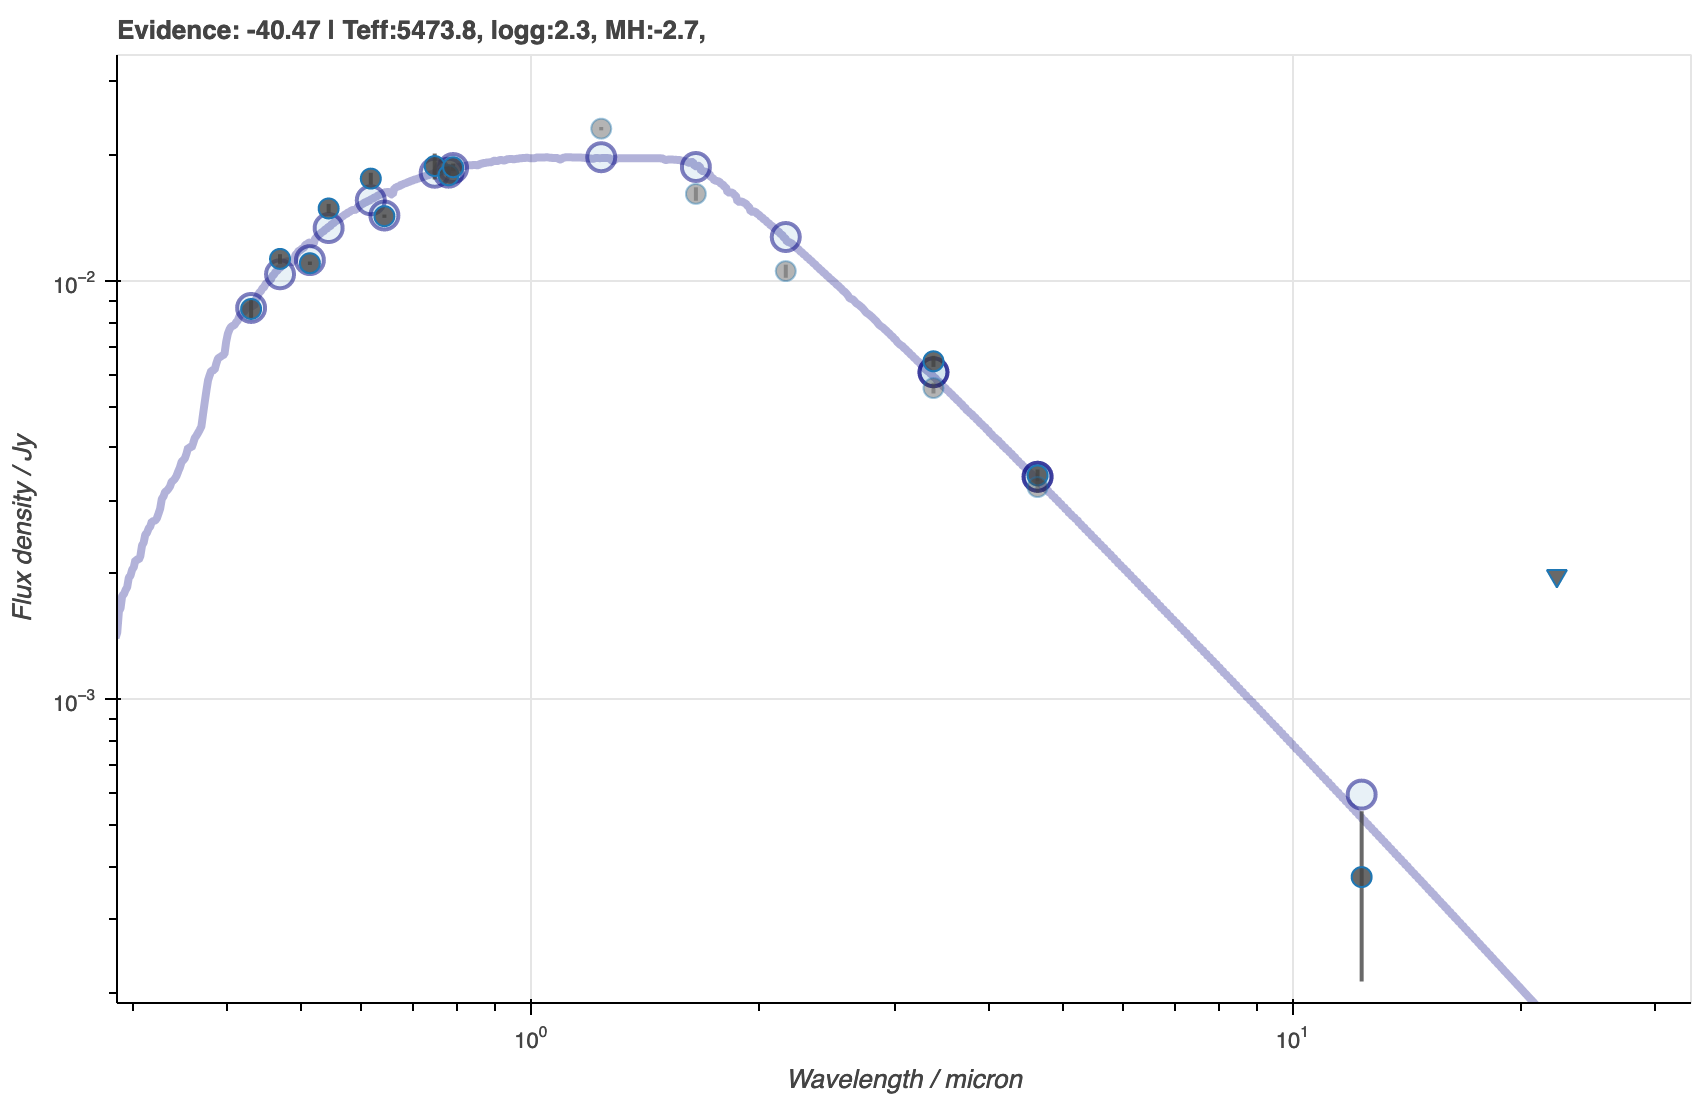
\includegraphics[width=\hsize]{figures/asassn-21qj-gmk-sed-fit.png}
      \caption{VOSA fit to photometry of ASAS-SN J0815 by gmk}
         \label{fig:sed}
\end{figure}



\begin{figure}
   \begin{centering}
   \includegraphics[width=\hsize]{figures/filter_curves.pdf}
      \caption{Filter curves for all telescopes and filters used to observe ASASSN-21qj.}
      \label{fig:allfilters}
      \script{plot_filter_curves.py}
      \end{centering}
\end{figure}



\subsection{Possible multiplicity in the  system}

Another star (Gaia EDR3 5539970601632026752) has a distance consistent (within uncertainties) with that of ASASSN-21qj.
%
This source has a cooler effective temperature.
%
It is about 3.8 arcseconds away from the primary star, with a distance of 560pc this is a projected distance of 2100au.
%
The primary star shows a value of RUWE of 1.10, implying that there is a substellar companion to the primary star.

Proper motions of the two stars are not consostent with each other, but if the primary has a substellar companion then this could change the measured proper motion of the primary and they could still be bound companions to each other.
%
TODO estimate the chance of having these two stars at the same distance but being unrelated to each other.

\section{Observations}\label{sec:obs}
An overview of all the photometry is presented in Figure~\ref{fig:allphot}.


\begin{figure*}
   \begin{centering}
   \includegraphics[width=\textwidth]{figures/eclipse_overview2.pdf}
      \caption{Photometry from the optical bands of the eclipse.
      %
The different telescopes and filters are indicated in the legend.
%
Each light curve is offset vertically by 0.8.
              }
        \label{fig:allphot}
        \script{plot_eclipse_overview2.py}
    \end{centering}
\end{figure*}



\subsection{ASAS-SN photometry}

The beginning of the eclipse was identified in \citet{RizzoSmith21} through the ASAS-SN survey.
%

\subsection{NEOWISE photometry}

The NEOWISE photometry is presented with the ASASSN $q$ light curve in Figure~\ref{fig:wisephot}.

\begin{figure*}
   \begin{centering}
   \includegraphics[width=\textwidth]{figures/all_photometry.png}
      \caption{NEOWISE $W1$ and $W2$ photometry of the star, with the WISE color in the lowest panel.
      %
      The $NEOWISE$ color changes from colourless to very red, which fades back towards colourless over $\sim 500$ days.
              }
              \label{fig:wisephot}
              \script{plot_all_photometry.py}
              \end{centering}
       \end{figure*}




NEOWISE....

\variable{output/collision_epoch_text.txt}


\subsection{LCOGT photometry}

\subsection{ATLAS}

ATLAS photometry was obtained from their database.



ATLAS is a project that searches for near earth asteroids down to a magnitude of 19 
\citep{Tonry18}.
%
Two filters were obtained, the `o' and `c' filters respectively.
%
Photometry consists of two to four photometric points observed each night when conditions permitted.
%
Photometry with large errors was rejected in a first pass.
%
The remaining observations during a night were averaged and an error based on the r.m.s. of these nightly points was calaulated.
%
The photometry covers the time period where the collision event occurred. 


\section{Analysis}\label{sec:dustcloud}

\subsection{Dust properties from the colors in the optical}



\begin{figure*}
   \begin{centering}
   \includegraphics[width=\textwidth]{figures/scale_combined_photometry.pdf}
      \caption{Photometry from the optical bands of the eclipse scaled arbitrarily so as to combine the light curves into a ``gray'' light curve.
      %
      The axis is inverted to show Absorption.
              }
              \label{fig:allphot}
              \script{plot_scale_combined_photometry.py}
              \end{centering}
       \end{figure*}



\section{Discussion}\label{sec:discussion}

Cound be a ring system

Could be a planetessimal system evolving

Alternatives?

%------------------------
\section{Conclusions}\label{sec:conclusion}

   \begin{enumerate}
      \item There was a collision between planetoids towards ASASSN-21qj which generated a debris cloud.
      \item The cloud moved in front of the star, and we have a fresh measure of the debris from a collision.
   \end{enumerate}

\begin{acknowledgements}
Thank matplotlib

\end{acknowledgements}

\bibliographystyle{aa}
\bibliography{bib}

\end{document}
